% Informe de modelado de NotifyHub. Compilar desde esta carpeta con: latexmk -lualatex notifyhub.tex
\documentclass[11pt,a4paper]{article}
\usepackage{fontspec}
\usepackage[spanish,es-noshorthands,es-tabla]{babel}
\usepackage[margin=2.2cm]{geometry}
\usepackage{graphicx}
\usepackage{float}
\usepackage{booktabs}
\usepackage{tabularx}
\usepackage{xcolor}
\usepackage{enumitem}
\usepackage{caption}
\usepackage[hidelinks]{hyperref}
\usepackage{titlesec}
\usepackage{fancyhdr}
\usepackage{parskip}

\setmainfont{Helvetica Neue}
\setmonofont{Menlo}[Scale=0.85]
\definecolor{indigo}{HTML}{4F46E5}
\definecolor{tinta}{HTML}{0F172A}
\titleformat{\section}{\Large\bfseries\color{indigo}}{\thesection}{0.8em}{}
\titleformat{\subsection}{\large\bfseries\color{tinta}}{\thesubsection}{0.8em}{}
\graphicspath{{../diagrams/render/}{../screens/}}
\setlist{itemsep=2pt,topsep=4pt}
\captionsetup{font=small,labelfont=bf}
\renewcommand{\arraystretch}{1.25}

\pagestyle{fancy}
\fancyhf{}
\fancyhead[L]{\small NotifyHub · Modelado y arquitectura}
\fancyhead[R]{\small Arquitectura de Software}
\fancyfoot[C]{\small\thepage}

\newcommand{\fig}[3][\textwidth]{%
  \begin{figure}[H]\centering
    \includegraphics[width=#1,height=0.78\textheight,keepaspectratio]{#2}
    \caption{#3}
  \end{figure}}

\begin{document}

\begin{titlepage}
  \centering
  \vspace*{3cm}
  {\Huge\bfseries\color{indigo} NotifyHub\par}
  \vspace{0.4cm}
  {\Large Servicio de Notificaciones y Registro Multicanal\par}
  \vspace{1.2cm}
  {\large Elementos de modelado, arquitectura implementada y metodología\par}
  \vspace{2.5cm}
  {\large Arquitectura de Software\par}
  \vspace{1.5cm}
  \begin{tabular}{rl}
    José Raúl Soriano Cazabal & Encargado del proyecto y líder técnico \\
    Andreea Margarita Maldonado Morales & Especialista del proyecto \\
  \end{tabular}
  \vfill
  {\small Repositorio: \texttt{github.com/joseraulsoriano/notifyhub} · Tablero: Jira, proyecto SCRUM\par}
  {\small Octubre de 2026\par}
\end{titlepage}

\tableofcontents
\newpage

%=====================================================================
\section{¿Qué es NotifyHub?}

NotifyHub es un servicio que recibe solicitudes de notificación de otras aplicaciones (un ERP, una tienda en línea,
una app móvil) y se encarga de que el mensaje llegue al destinatario por el canal adecuado: correo (SendGrid), SMS
(Twilio), notificación push (Firebase Cloud Messaging) o webhook. Si el canal principal falla, reintenta con espera
exponencial y, cuando se agota, \textbf{conmuta a un canal secundario} (\emph{fallback}). Cada intento y cada cambio
de estado queda en una bitácora de auditoría que solo admite inserciones.

El proyecto está construido alrededor de tres patrones GoF que se pueden señalar en el código:
\textbf{Factory Method} (crear el emisor de cada proveedor), \textbf{Strategy} (elegir proveedor por costo, prioridad
o disponibilidad) y \textbf{Observer} (publicar cada cambio de estado a quien le interese).

\subsection{Requisitos funcionales}
\begin{tabularx}{\textwidth}{@{}lX@{}}
\toprule
\textbf{RF} & \textbf{Descripción} \\
\midrule
RF1 & Recibir solicitudes por REST con API key, validarlas, deduplicarlas por \texttt{Idempotency-Key} y encolarlas por prioridad. \\
RF2 & Enrutar cada solicitud al proveedor de su canal mediante factorías configurables (Factory Method). \\
RF3 & Seleccionar proveedor dinámicamente (Strategy) y conmutar a un canal secundario cuando el principal falla. \\
RF4 & Registrar cada intento y transición en una bitácora de auditoría consultable y exportable. \\
RF5 & Notificar los cambios de estado a servicios suscriptores (Observer + outbox transaccional). \\
\bottomrule
\end{tabularx}

\subsection{Requisitos no funcionales}
\begin{itemize}
  \item \textbf{Confiabilidad:} ninguna solicitud aceptada se pierde; se persiste antes de encolarse.
  \item \textbf{Idempotencia:} reenviar la misma solicitud no duplica el envío (ventana de 24 h).
  \item \textbf{Rendimiento:} meta de 1,000 notificaciones/min con p95 de aceptación menor a 200 ms.
  \item \textbf{Seguridad:} API key por cliente, límite de solicitudes por minuto y enmascarado de datos personales.
  \item \textbf{Costo:} operar en el plan gratuito de Cloudflare (0 USD).
  \item \textbf{Mantenibilidad:} el dominio no depende de ningún framework; cambiar de infraestructura no toca la lógica.
\end{itemize}

%=====================================================================
\section{Metodología: Scrum}

El proyecto se gestiona con \textbf{Scrum} adaptado a un equipo de dos personas. Se eligió porque el alcance se
descompone de forma natural en requisitos funcionales independientes (RF1 a RF5) que se pueden entregar uno por
sprint, y porque la entrega de avance y la entrega final funcionan como revisiones de sprint con el profesor.

\subsection{Roles}
\begin{tabularx}{\textwidth}{@{}lX@{}}
\toprule
\textbf{Rol Scrum} & \textbf{Quién y qué hace} \\
\midrule
Product Owner & José Raúl Soriano. Define alcance, prioriza el backlog y acepta historias. \\
Scrum Master / líder técnico & José Raúl Soriano. Coordina, quita bloqueos, cuida la arquitectura y el CI/CD. \\
Equipo de desarrollo & José Raúl Soriano (plataforma, API, infraestructura) y Andreea Maldonado (dominio y patrones GoF, proveedores, auditoría, calidad). \\
Cliente / revisor & El profesor de la materia, en las entregas de avance y final. \\
\bottomrule
\end{tabularx}

\subsection{Sprints y entregables}
Cinco sprints de dos semanas (del 28 de septiembre al 4 de diciembre de 2026). Cada sprint tiene un objetivo ligado
a un requisito funcional; el backlog suma \textbf{41 historias y 142 puntos de historia}, repartidos en unos 27--31
puntos por sprint.

\begin{tabularx}{\textwidth}{@{}llXr@{}}
\toprule
\textbf{Sprint} & \textbf{Fechas} & \textbf{Objetivo} & \textbf{SP} \\
\midrule
S0 · Planeación & 28 sep -- 9 oct & Requisitos, ADRs, modelos, diagramas, contrato OpenAPI y riesgos & 27 \\
S1 · RF1 & 12 -- 23 oct & Monorepo, entorno local, CI, recepción y consulta de notificaciones & 27 \\
S2 · RF2 & 26 oct -- 6 nov & Factory Method, adaptadores de proveedores y despachador & 27 \\
S3 · RF3 + RF4 & 9 -- 20 nov & Strategy, fallback, circuit breaker y bitácora & 31 \\
S4 · RF5 & 23 nov -- 4 dic & Observer, outbox, dashboards, pruebas de carga y entrega final & 30 \\
\bottomrule
\end{tabularx}

\fig{00-cronograma.png}{Cronograma por sprint y épica.}

\subsection{Artefactos y ceremonias}
\begin{itemize}
  \item \textbf{Product backlog} en Jira (proyecto SCRUM), organizado en 8 épicas: planeación, plataforma y DevOps,
        RF1 a RF5, y calidad y entrega. Cada historia lleva responsable, puntos, prioridad y criterios de aceptación.
        El backlog también está versionado en el repositorio (\texttt{docs/planeacion/backlog.json}).
  \item \textbf{Sprint planning} al inicio de cada sprint: se toman las historias de mayor prioridad del RF del sprint.
  \item \textbf{Seguimiento} en el tablero de Jira; cada commit lleva la clave de la historia, así Jira enlaza el código
        con la historia automáticamente.
  \item \textbf{Sprint review} en las entregas al profesor; el avance por historia se publica en \texttt{docs/avance.md}
        con evidencia (archivo, prueba o diagrama).
  \item \textbf{Retrospectiva} al cierre: por ejemplo, tras el Sprint 0 se decidió migrar a Cloudflare Workers nativo
        (ADR-007) para no pagar infraestructura.
\end{itemize}

\subsection{Definition of Done}
Una historia está terminada cuando: (1) sus criterios de aceptación están cubiertos por al menos una prueba
automatizada, (2) el CI está en verde, (3) la otra persona revisó y aprobó el pull request y (4) la documentación
está al día (OpenAPI, ADR o README).

\subsection{Prácticas de ingeniería que sostienen la metodología}
\begin{itemize}
  \item \textbf{Ramas cortas por historia} (\texttt{SCRUM-22-adaptador-sendgrid}) y pull request con revisión cruzada.
  \item \textbf{Conventional Commits} con la clave de Jira (\texttt{feat(api): SCRUM-22 \dots}), validados con Husky
        y commitlint.
  \item \textbf{Integración continua} en GitHub Actions: lint, tipos, pruebas, build y una prueba de humo contra
        Postgres real en cada pull request.
  \item \textbf{Registro de decisiones (ADR):} cada decisión de arquitectura queda escrita con contexto, decisión,
        consecuencias y alternativas descartadas. Hay 7 ADR; una aceptada no se edita, se sustituye por otra.
  \item \textbf{Gestión de riesgos:} matriz de 10 riesgos con probabilidad, impacto, mitigación y disparador
        (\texttt{docs/riesgos-y-pruebas.md}).
\end{itemize}

%=====================================================================
\section{Arquitectura implementada}

\subsection{Estilo: hexagonal (puertos y adaptadores) orientada a eventos y \emph{serverless}}

La arquitectura combina tres ideas:

\begin{enumerate}
  \item \textbf{Hexagonal (puertos y adaptadores).} El centro es el \emph{dominio} (\texttt{packages/domain}:
        entidades, máquina de estados y errores, sin dependencias) y la \emph{aplicación}
        (\texttt{packages/application}: casos de uso, puertos y los patrones de despacho). Todo lo que toca el mundo
        exterior es un \emph{adaptador} que implementa un puerto: el repositorio en Postgres, la cola, el limitador
        de solicitudes, los emisores de cada proveedor. ESLint impide que el dominio importe infraestructura.
  \item \textbf{Asíncrona, orientada a mensajes.} La API solo acepta y encola (responde \texttt{202 Accepted}); el
        envío real lo hace un proceso separado, el despachador, que consume tres colas por prioridad. Así un proveedor
        lento nunca bloquea a quien llama.
  \item \textbf{Serverless en el borde.} Todo corre en Cloudflare Workers del plan gratuito: API y despachador son
        Workers, las colas son Cloudflare Queues, el límite de solicitudes es un Durable Object y la base de datos
        es Postgres (Neon) a través de Hyperdrive.
\end{enumerate}

La prueba de que la hexagonal funciona: entre el Sprint 0 y el Sprint 1 se cambió NestJS por Hono, BullMQ/Redis por
Cloudflare Queues y Prisma Client por \texttt{pg}, y los casos de uso y sus pruebas \textbf{no cambiaron} (ADR-007).

\subsection{Capas y monorepo}
\begin{tabularx}{\textwidth}{@{}lX@{}}
\toprule
\textbf{Paquete} & \textbf{Responsabilidad} \\
\midrule
\texttt{packages/domain} & Entidades, estados y errores. No depende de nada. \\
\texttt{packages/application} & Casos de uso, puertos y despacho (Strategy, Factory Method, Observer). \\
\texttt{packages/providers} & Emisores por proveedor (Template Method) y sus creadores (Factory Method). \\
\texttt{packages/persistence} & Esquema y migraciones Prisma; repositorios con \texttt{pg}. \\
\texttt{packages/client}, \texttt{ui} & SDK de TypeScript y componentes React reutilizables. \\
\texttt{apps/api} & Worker Hono: recepción, consulta, proveedores y bitácora. \\
\texttt{apps/dispatcher} & Worker consumidor de colas: despacho, reintentos y fallback. \\
\texttt{apps/console} & Consola web (Astro + React) para operar el sistema. \\
\bottomrule
\end{tabularx}

\medskip
Monorepo con pnpm workspaces y Turborepo, TypeScript estricto. Stack: Hono, Cloudflare Workers/Queues/Durable
Objects/Hyperdrive, PostgreSQL con Prisma, Astro + React + shadcn/ui, Vitest, GitHub Actions.

\subsection{Patrones de diseño}
\begin{tabularx}{\textwidth}{@{}lX@{}}
\toprule
\textbf{Patrón} & \textbf{Dónde y para qué} \\
\midrule
Factory Method & \texttt{SenderCreator} y \texttt{SenderRegistry}: crean el emisor concreto de cada proveedor sin que el despachador conozca las clases concretas. Agregar un proveedor es agregar un creador. \\
Strategy & \texttt{CostStrategy}, \texttt{PriorityStrategy}, \texttt{AvailabilityStrategy}: ordenan los proveedores de un canal; la estrategia se elige según la prioridad de la notificación. \\
Observer & \texttt{EventPublisher}: cada cambio de estado e intento se publica; suscriptores como la bitácora, métricas y el outbox reaccionan sin acoplarse al despachador. \\
Template Method / Adapter & \texttt{BaseSender} fija el algoritmo (validar, enviar, mapear respuesta) y cada proveedor implementa solo \texttt{doSend}. \\
Chain of Responsibility & \texttt{FallbackPolicy}: arma la cadena de canales (preferido $\rightarrow$ secundarios) por la que pasa la notificación. \\
\bottomrule
\end{tabularx}

\subsection{Diagrama de contexto}
NotifyHub como caja negra: quién lo usa y con quién habla.
\fig[0.95\textwidth]{01-contexto.png}{Diagrama de contexto (C4 nivel 1).}

\subsection{Diagrama de contenedores}
Los procesos y almacenes que forman el sistema. Los clientes llaman a la API, que persiste en PostgreSQL y encola en
Queues; el despachador consume la cola y llama a los proveedores; el \emph{event relay} (Sprint 4) leerá el outbox y
entregará eventos a los suscriptores. Las líneas punteadas son telemetría (OpenTelemetry).
\fig[0.85\textwidth]{02-contenedores.png}{Diagrama de contenedores (C4 nivel 2).}

\subsection{Diagrama de despliegue (arquitectura implementada)}
Lo que está desplegado hoy en Cloudflare: tres Workers (consola, API y despachador), un Durable Object para el límite
de solicitudes, tres colas por prioridad y Hyperdrive como pool de conexiones hacia Neon Postgres. El código vive en
GitHub, donde Actions corre el CI en cada pull request; el despliegue se hace con \texttt{wrangler deploy}.
\fig{07-despliegue.png}{Despliegue en Cloudflare (plan gratuito).}

\paragraph{Funcionamiento de punta a punta.}
\begin{enumerate}
  \item Una aplicación cliente hace \texttt{POST /v1/notifications} con su API key y, opcionalmente, una
        \texttt{Idempotency-Key}.
  \item El Worker de la API valida la llave, consulta al Durable Object si el cliente está dentro de su límite,
        valida el cuerpo y revisa la idempotencia.
  \item Guarda la notificación en Postgres con estado \texttt{RECEIVED}, la encola en la cola de su prioridad, la
        pasa a \texttt{QUEUED} y responde \texttt{202} con el \texttt{id}.
  \item El Worker despachador toma el mensaje, la \texttt{FallbackPolicy} arma la cadena de canales, la Strategy ordena
        los proveedores y el \texttt{SenderRegistry} crea el emisor.
  \item Si el proveedor falla de forma transitoria se reintenta hasta 3 veces con backoff exponencial; si se agota,
        pasa al siguiente proveedor o canal. Cada intento se guarda y se publica como evento.
  \item El cliente o el operador consultan el estado con \texttt{GET /v1/notifications/\{id\}} o en la consola, que
        dibuja la ruta del mensaje: cada canal es una línea, cada intento una estación y cada fallback un transbordo.
\end{enumerate}

\paragraph{Qué es real y qué es simulado.} Es real la recepción con idempotencia y límite de solicitudes, las colas
por prioridad, la máquina de estados, los reintentos, el fallback, la bitácora en Postgres, la API, el SDK y la
consola. Los proveedores están \textbf{simulados}: su comportamiento depende de su salud configurada (\texttt{UP},
\texttt{DEGRADED}, \texttt{DOWN}), lo que permite demostrar el fallback sin credenciales. Outbox y suscripciones
(RF5) y circuit breaker están planeados para S3--S4.

%=====================================================================
\section{Diagrama de casos de uso}

Actores humanos a la izquierda (aplicación cliente, operador, administrador) y sistemas externos a la derecha
(cola/despachador, proveedores y suscriptores). Las relaciones \guillemotleft include\guillemotright{} son pasos
obligatorios (toda llamada se autentica; todo despacho reintenta y publica eventos); las
\guillemotleft extend\guillemotright{} son opcionales (la deduplicación solo ocurre si llega
\texttt{Idempotency-Key}; el fallback solo si se agota el canal; exportar CSV es opcional al consultar la bitácora).

\fig{08-casos-de-uso.png}{Diagrama de casos de uso.}

\begin{tabularx}{\textwidth}{@{}llX@{}}
\toprule
\textbf{CU} & \textbf{Actor} & \textbf{Descripción breve} \\
\midrule
CU-01 & App cliente & Envía una notificación con remitente, destinatario, mensaje, prioridad y canal preferido. \\
CU-04 & App cliente, operador & Consulta estado, intentos e historial de una notificación. \\
CU-05 & Operador & Lista notificaciones filtrando por estado, canal y prioridad, con paginación. \\
CU-06 & Despachador & Entrega la notificación por el mejor proveedor del canal. \\
CU-08 & Despachador & Conmuta al canal secundario cuando el principal se agota. \\
CU-09/10 & Operador & Consulta la bitácora de auditoría y la exporta a CSV. \\
CU-11 & Administrador & Habilita proveedores y cambia su salud, lo que afecta el ruteo en vivo. \\
CU-13/14 & Administrador, suscriptor & Gestiona suscripciones y recibe eventos de cambio de estado (S4). \\
\bottomrule
\end{tabularx}

%=====================================================================
\section{Diagramas de flujo}

\subsection{Recepción de una notificación (RF1)}
Las validaciones van de la más barata a la más cara: llave, límite, esquema e idempotencia. Lo importante del diseño
es que la notificación se \textbf{persiste antes de encolarse}: si la cola falla, queda en \texttt{RECEIVED} y el
despachador la recupera en un barrido, así nunca se pierde.
\fig[0.72\textwidth]{09-flujo-recepcion.png}{Flujo de recepción en la API.}

\subsection{Despacho con reintentos y fallback (RF2, RF3)}
Es el algoritmo del \texttt{DispatchService}. Por cada canal de la cadena, la Strategy ordena los proveedores y la
factoría crea el emisor. Un error transitorio provoca reintentos con backoff; un error permanente o los reintentos
agotados pasan al siguiente proveedor y, después, al siguiente canal. Como Queues entrega \emph{al menos una vez}, lo
primero que hace es verificar que la notificación siga en \texttt{QUEUED}.
\fig[0.62\textwidth]{10-flujo-despacho.png}{Flujo de despacho en el Worker despachador.}

%=====================================================================
\section{Diagrama entidad-relación}

\texttt{NOTIFICATION} es la entidad central: pertenece a un \texttt{CLIENT\_APP}, tiene muchos
\texttt{DELIVERY\_ATTEMPT} (cada uno hecho por un \texttt{PROVIDER}) y deja registros en \texttt{AUDIT\_LOG}.
\texttt{ROUTING\_RULE} define el orden de proveedores y el canal de fallback por prioridad. Para RF5,
\texttt{OUTBOX\_EVENT} guarda los eventos en la misma transacción que el cambio de estado, y
\texttt{SUBSCRIPTION\_DELIVERY} registra la entrega de cada evento a cada suscripción. La llave
\texttt{(client\_app\_id, idempotency\_key)} es única para garantizar la deduplicación.
\fig{04-er.png}{Modelo entidad-relación.}

%=====================================================================
\section{Diagrama de secuencia}

Envío de una notificación con los tres desenlaces posibles: éxito directo, error transitorio con reintento y
fallback a un proveedor secundario. Muestra cómo colaboran los patrones: el \texttt{DispatchService} pide el orden a
la Strategy, el emisor a la factoría y publica cada cambio al \texttt{EventPublisher} (Observer).
\fig[0.95\textwidth]{05-secuencia-envio.png}{Secuencia de envío con fallback.}

%=====================================================================
\section{Diagramas complementarios}

\subsection{Clases y patrones}
\fig{03-clases-patrones.png}{Diagrama de clases con Factory Method, Strategy y Observer.}

\subsection{Máquina de estados de la notificación}
Cada transición solo procede desde el estado esperado; eso hace idempotente al despachador.
\fig[0.6\textwidth]{06-estados.png}{Estados de una notificación.}

%=====================================================================
\section{Diagrama de navegación}

La consola web (\texttt{apps/console}) tiene seis pantallas agrupadas en la barra lateral: \emph{Operación}
(Resumen, Notificaciones, Nueva solicitud), \emph{Configuración} (Proveedores y ruteo, Suscripciones) y
\emph{Control} (Bitácora). Sin conexión guardada arranca en modo demo con un cliente simulado; desde el diálogo
\emph{Conectar} se pasa a la API real. El panel de detalle muestra la ruta del mensaje y enlaza con la bitácora
filtrada por esa notificación.
\fig[0.8\textwidth]{11-navegacion.png}{Diagrama de navegación de la consola.}

\begin{figure}[H]\centering
  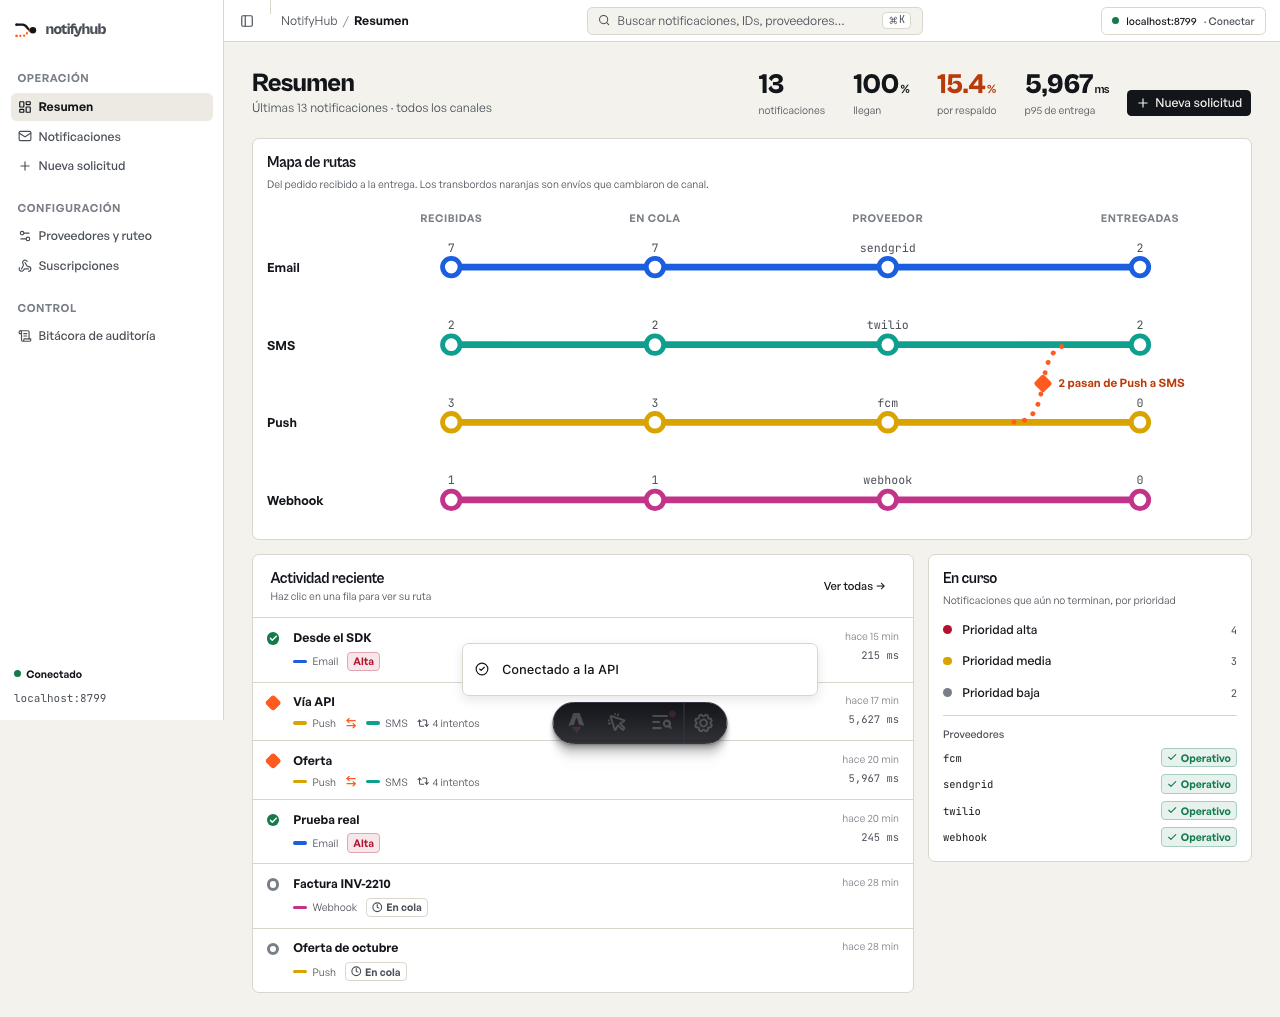
\includegraphics[width=0.49\textwidth]{01-resumen.png}\hfill
  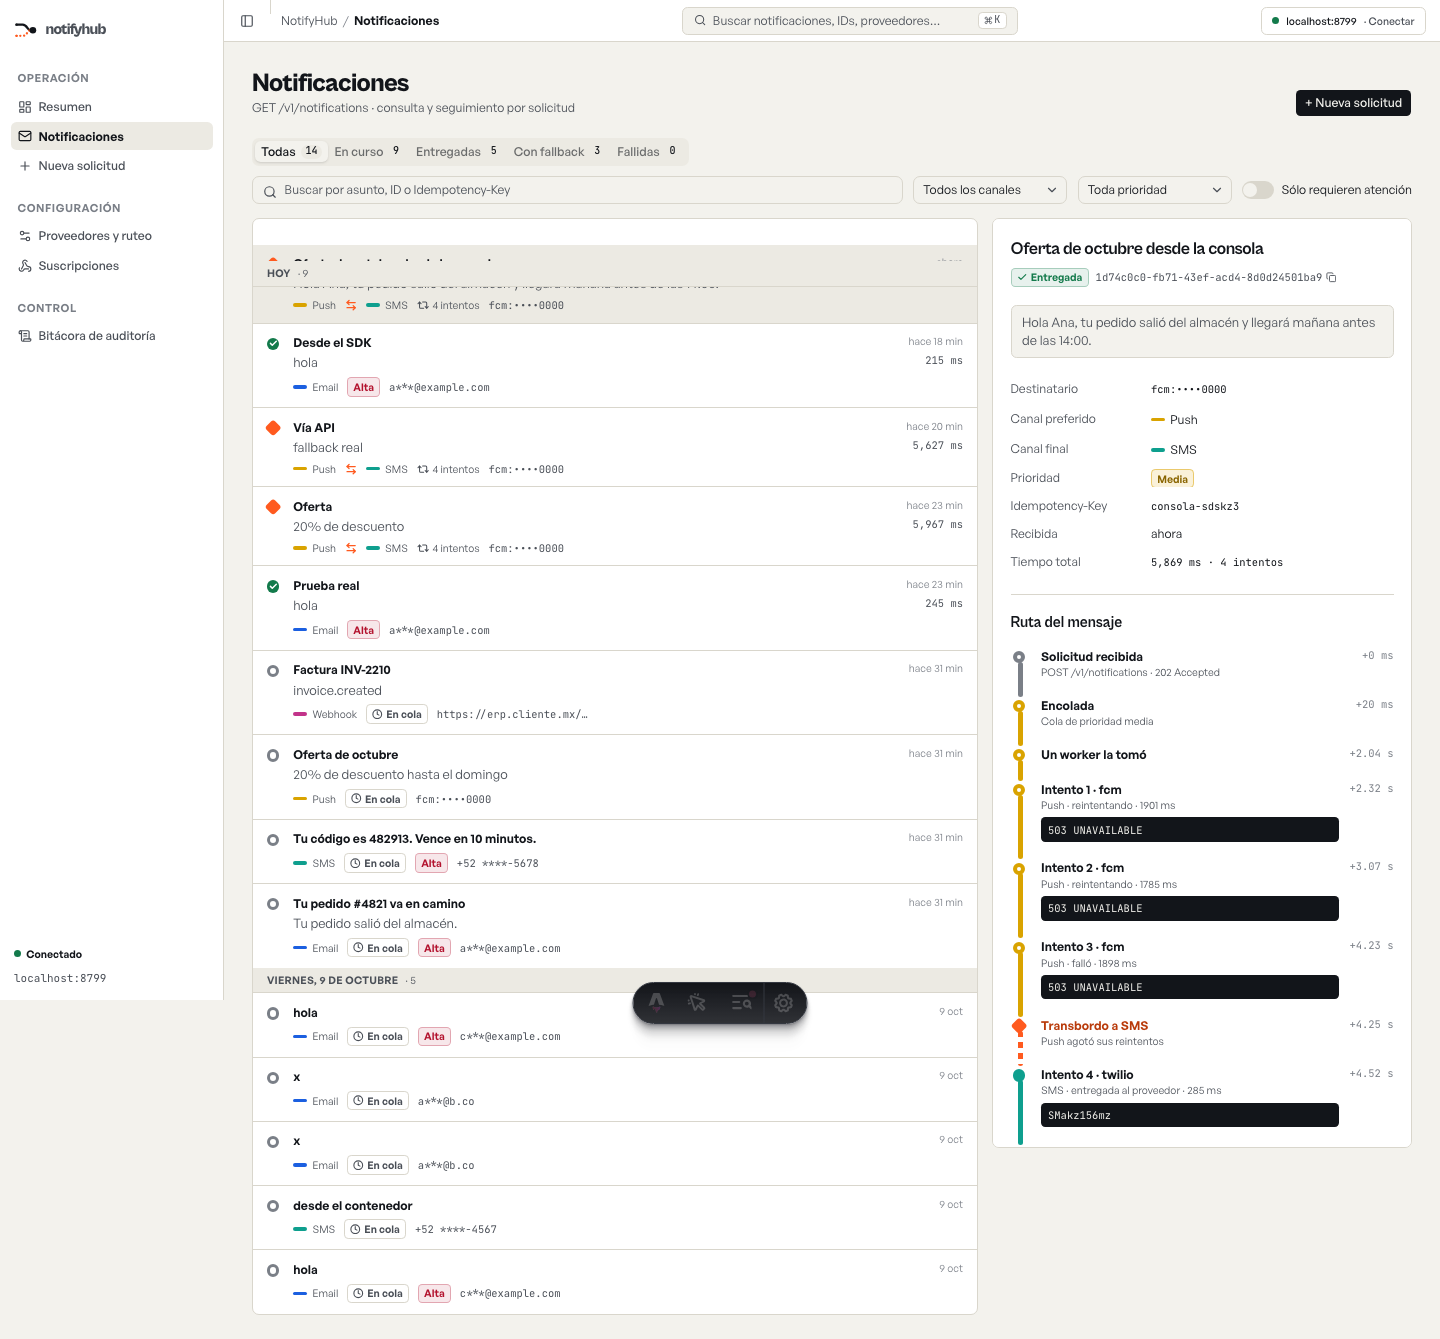
\includegraphics[width=0.49\textwidth]{02-notificacion-fallback.png}
  \caption{Pantallas Resumen y detalle de una notificación con fallback (tres intentos en Push y transbordo a SMS).}
\end{figure}
\begin{figure}[H]\centering
  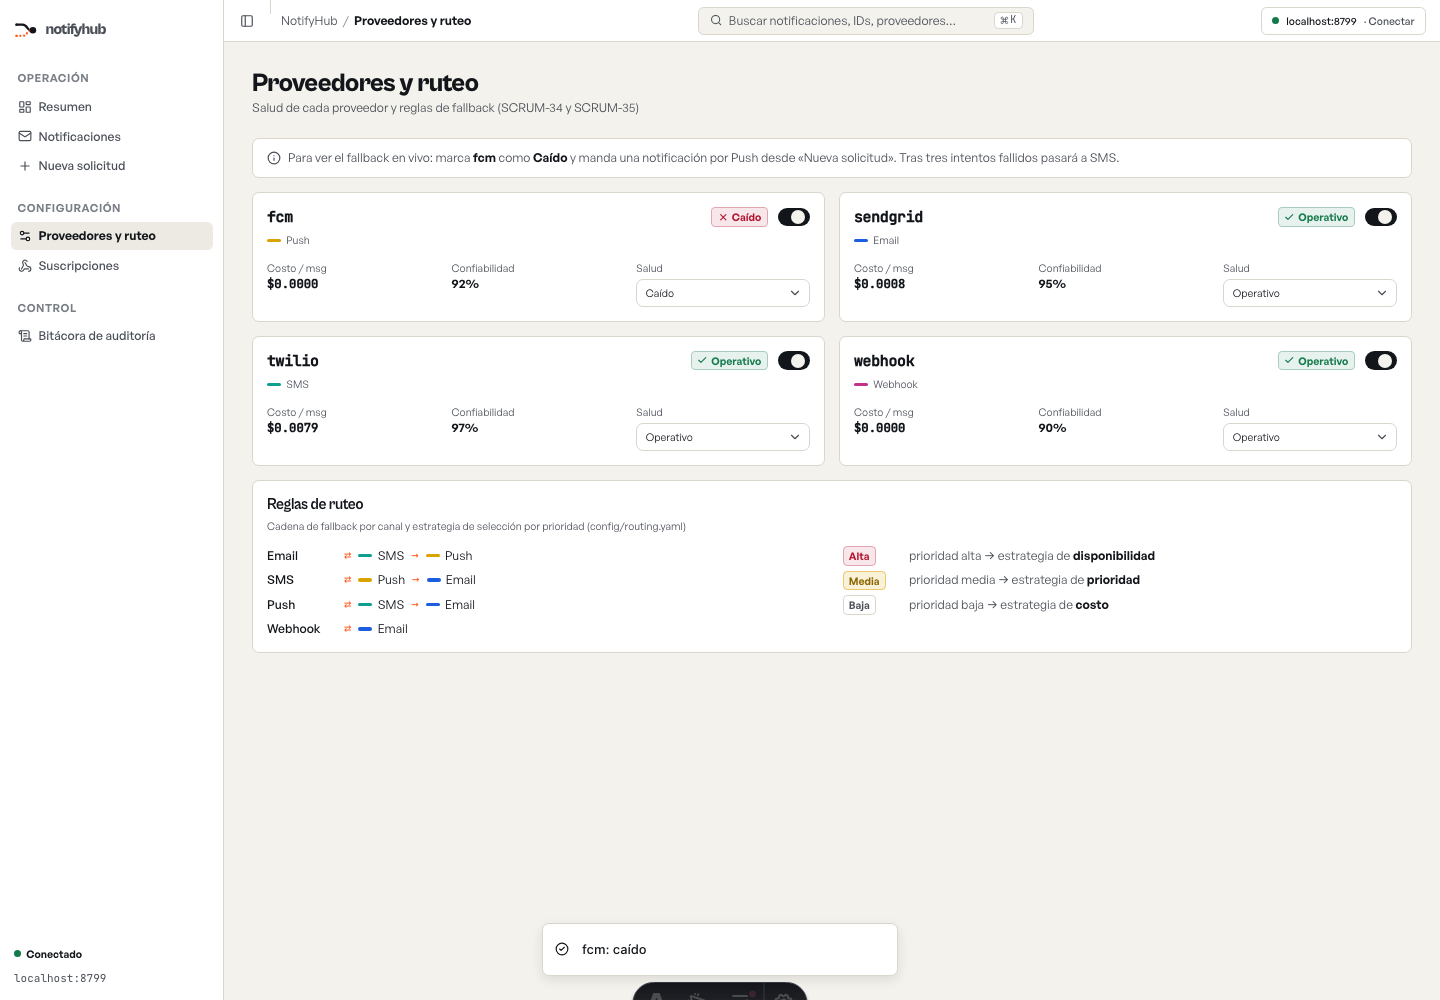
\includegraphics[width=0.49\textwidth]{03-proveedores.png}\hfill
  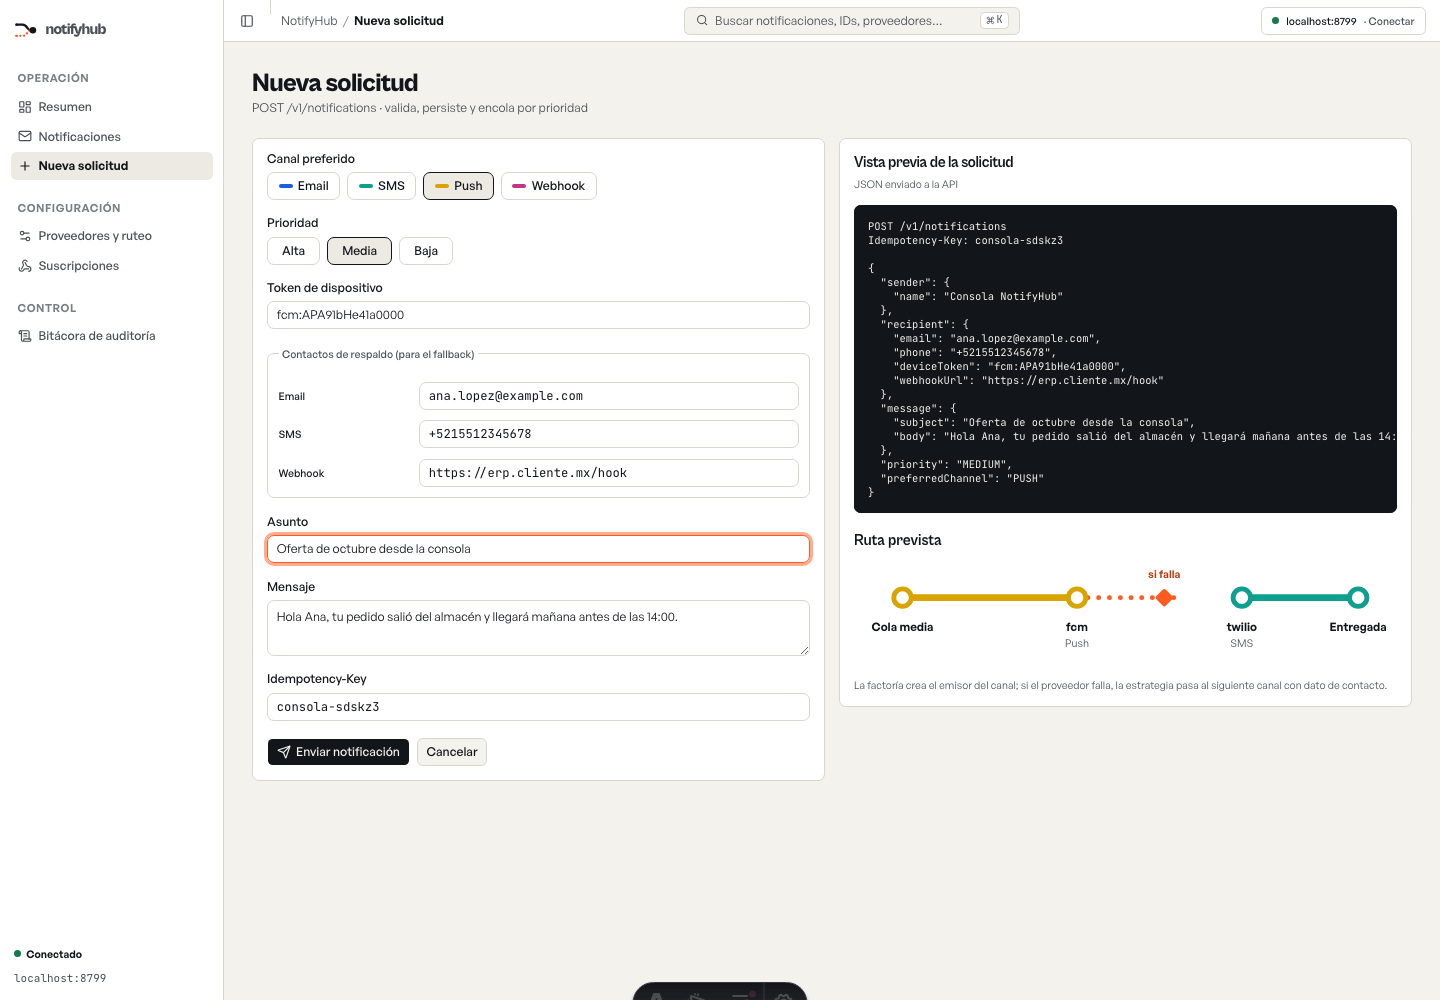
\includegraphics[width=0.49\textwidth]{04-nueva-solicitud.png}
  \caption{Pantallas Proveedores y ruteo, y Nueva solicitud.}
\end{figure}

%=====================================================================
\section{Calidad y estado actual}

\begin{itemize}
  \item \textbf{148 pruebas automatizadas en verde} (Vitest) en dominio, aplicación, proveedores, API, SDK, UI y
        consola, más una prueba de humo contra Postgres real en CI.
  \item Pirámide de pruebas: unitarias (máquina de estados, casos de uso, estrategias, fallback), de componente
        (cada código de respuesta del contrato OpenAPI), integración, humo y carga con k6 (S4).
  \item Contrato de la API en OpenAPI 3.1 (\texttt{docs/api/openapi.yaml}), validado con Redocly.
  \item Desplegado y verificado en Cloudflare: API, despachador y consola.
  \item Pendiente: adaptadores reales de proveedores, circuit breaker, outbox y suscripciones (RF5), dashboards y
        prueba de carga.
\end{itemize}

\end{document}
